\newpage
\appendix

This appendix includes: 
\begin{itemize}
    \item Related work discussion (Appendix~\ref{sec:related works}).
    \item Detailed comparisons of \textit{Lens} against state-of-the-art models on OneIG, GenEval, LongText (EN), and CVTG (Appendix~\ref{sec:benchmark-details}).
    \item Reasoner analysis (Appendix~\ref{sec:various reasoners}).
    \item Rubric visualizations and training-data visualizations (Appendix~\ref{sec:visualization-appendix}).
    \item Implementation details (Appendix~\ref{sec:implementation details}).
    \item All prompts used in this work (Appendix~\ref{sec:all-prompts}).
    \item Broader impacts and limitations of this work (Appendix~\ref{sec:limitations}).
\end{itemize}


\section{Related Works}
\label{sec:related works}

\subsection{Foundational T2I Models}
Text-to-image (T2I) foundation models have progressed from latent diffusion models to large-scale diffusion Transformers, rectified-flow models, and proprietary multimodal image-generation systems. Early latent diffusion models (LDMs), including Stable Diffusion, established the paradigm of performing generation in a compressed latent space, substantially reducing training and inference costs compared with pixel-space diffusion~\citep{rombach2022high}. Building on this paradigm, SDXL further improves high-resolution synthesis through a larger UNet, stronger text conditioning, multi-aspect-ratio training, and a dedicated refinement stage~\citep{podell2024sdxl}.

More recent models have shifted toward Transformer-based backbones and rectified-flow objectives. Stable Diffusion 3 and its 3.5 variants adopt MMDiT-style architectures with rectified-flow training~\citep{esser2024scaling,stabilityai2024sd35}, following the broader trend of scalable diffusion Transformers~\citep{peebles2023scalable}. Recent open-source and commercial systems, such as FLUX~\citep{flux2024}, SANA~\citep{xie2024sana}, HiDream-I1~\citep{cai2025hidream}, Qwen-Image~\citep{wu2025qwenimage}, Hunyuan-Image-3.0~\citep{cao2025hunyuanimage}, Z-Image~\citep{cai2025zimage}, GPT Image~\citep{openai2025gptimage}, Gemini 2.5 Flash Image (Nano Banana)~\citep{google2025nanobanana}, Kolors 2.0~\citep{kolors2}, and Seedream 4.0~\citep{seedream2025seedream4}, further advance visual quality, prompt following, text rendering, image editing, reference consistency, and inference efficiency.

In parallel, unified multimodal and autoregressive generators aim to integrate image synthesis with language modeling and visual understanding. Janus-Pro~\citep{chen2025januspro} scales a unified autoregressive framework for both multimodal understanding and generation. Transfusion~\citep{zhou2024transfusion} combines next-token prediction with diffusion over continuous image representations, while BAGEL~\citep{deng2025BAGEL} scales decoder-only multimodal pretraining on interleaved text, image, video, and web data. Although these approaches achieve strong performance and broaden the capabilities of T2I systems, they often require increasingly large models, massive training data, and complex system designs. This trend motivates our study of efficient foundation-model training, aiming to achieve competitive generation quality with substantially reduced computational cost.

\subsection{Post-training for T2I Models}

Post-training has become an important stage for improving the alignment and generation quality of T2I models. Early efforts mainly relied on supervised fine-tuning, while recent work has increasingly explored preference-based optimization and reinforcement learning (RL). These methods aim to improve model behavior beyond likelihood-based pre-training by directly optimizing for human preferences, reward-model judgments, or task-specific generation criteria.

One major line of work adapts direct preference optimization (DPO) to diffusion models. These methods train the model using positive-negative image pairs or preference sets, encouraging generations preferred by humans or reward models while suppressing less desirable outputs. Representative approaches include Diffusion-DPO~\citep{wallace2024diffusion}, D3PO~\citep{yang2024using}, SPO~\citep{liang2025aesthetic}, and related variants~\citep{yuan2024self,yang2024dense,li2024aligning,hong2026margin}. Compared with online RL, DPO-style methods are relatively simple and stable, as they optimize preference objectives without requiring explicit reward maximization during sampling.

Another line of work applies policy-gradient-based RL to the generation process. GRPO-based methods formulate image generation as a sequential decision-making problem and optimize the denoising or flow-matching trajectory directly. For flow-matching models, Flow-GRPO~\citep{liu2025flow} and its variants~\citep{li2025mixgrpo,wang2025pref} extend policy-gradient optimization to continuous generative dynamics by converting deterministic sampling into an equivalent stochastic formulation. Related methods, such as DiffusionNFT~\citep{zheng2025diffusionnft} and AWM~\citep{xue2025advantage}, further investigate RL objectives over the generative process, introducing online optimization frameworks and advantage-aware or negative-aware objectives to guide model improvement.

Across both preference-optimization and RL-based post-training, reward design is a critical factor. A useful reward should capture not only global aesthetic quality, but also prompt faithfulness, object correctness, spatial and compositional consistency, text rendering, and safety-related constraints. Poorly designed rewards may cause reward hacking, reduced diversity, or misalignment between the optimization objective and human preference. Therefore, recent work~\citep{feng2025rubricrl,gunjal2025rubrics,huang2025reinforcement,he2025advancedif} has increasingly emphasized fine-grained, multi-dimensional reward construction. This motivates our rubric-based post-training strategy, which provides explicit and structured evaluation criteria for RL optimization of T2I foundation models.


\begin{table*}[t]
  \centering
  \caption{Comparison of \textit{Lens} with commercial and open-source models on \textbf{OneIG (EN)}. The best results are highlighted in \textbf{bold}, and the second-best results are \underline{underlined}.}
  \vspace{1mm}
  \label{tab:main_oneig}
  \small
  \setlength{\tabcolsep}{4.8pt}
  \renewcommand{\arraystretch}{1.12}
  \resizebox{\textwidth}{!}{%
  \begin{tabular}{l|c|cccccc}
    \toprule
    Model & Size & Alignment & Text & Reasoning & Style & Diversity & Overall \\
    \midrule
    \multicolumn{8}{l}{\emph{Commercial models}} \\
    Kolors 2.0 & --
      & 0.820 & 0.427 & 0.262 & 0.360 & 0.300 & 0.434 \\
    Seedream 3.0 & --
      & 0.818 & 0.865 & 0.275 & 0.413 & 0.277 & 0.530 \\
    Seedream 4.0 & --
      & 0.892 & 0.983 & 0.347 & 0.453 & 0.191 & 0.573 \\
    GPT Image 1 [High] & --
      & 0.851 & 0.857 & 0.345 & 0.462 & 0.151 & 0.533 \\
    Nano Banana 2.0 & --
      & 0.888 & 0.944 & 0.334 & 0.481 & 0.245 & 0.578 \\
    \midrule
    \multicolumn{8}{l}{\emph{Open-source models}} \\
    Janus-Pro & 7B
      & 0.553 & 0.001 & 0.139 & 0.276 & \textbf{0.365} & 0.267 \\
    BAGEL & 14B
      & 0.769 & 0.244 & 0.173 & 0.367 & \underline{0.251} & 0.361 \\
    HiDream-I1-Full & 17B
      & 0.829 & 0.707 & 0.317 & 0.347 & 0.186 & 0.477 \\
    SD3.5 Large & 8B
      & 0.809 & 0.629 & 0.294 & 0.353 & 0.225 & 0.462 \\
    FLUX.1 [Dev] & 12B
      & 0.786 & 0.523 & 0.253 & 0.368 & 0.238 & 0.434 \\
    FLUX.2-Klein & 9B
      & \underline{0.887} & 0.866 & 0.312 & \textbf{0.442} & 0.156 & 0.532 \\
    Z-Image-Turbo & 6B
      & 0.840 & \textbf{0.994} & 0.298 & 0.368 & 0.139 & 0.528 \\
    Z-Image & 6B
      & 0.881 & \underline{0.987} & 0.280 & 0.387 & 0.194 & 0.546 \\
    Qwen-Image & 20B
      & 0.882 & 0.891 & 0.306 & \underline{0.418} & 0.197 & 0.539 \\
    \midrule
    \textbf{Lens-Turbo} & \textbf{3.8B}
      & 0.884 & 0.972 & \textbf{0.349} & 0.383 & 0.180 & \underline{0.554} \\
    \textbf{Lens} & \textbf{3.8B}
      & \textbf{0.891} & 0.960 & \underline{0.343} & 0.404 & 0.186 & \textbf{0.557} \\
    \bottomrule
  \end{tabular}%
  }
\end{table*}

\subsection{Distillation for T2I Models}

A central challenge of diffusion- and flow-based T2I models is their expensive iterative sampling process. Early acceleration methods mainly improve the inference solver without modifying model parameters. Representative examples include deterministic samplers such as DDIM~\citep{ddim}, as well as high-order ODE solvers such as DPM-Solver~\citep{dpmsolver} and UniPC~\citep{unipc}. Although these training-free methods can reduce the number of function evaluations, generation quality often degrades when the sampling budget becomes extremely small, especially for high-resolution text-conditioned synthesis under strong classifier-free guidance.


\begin{table*}[t]
  \centering
  \caption{Comparison of \textit{Lens} with commercial and open-source models on \textbf{GenEval}.}
  \vspace{1mm}
  \label{tab:main_geneval}
  \small
  \setlength{\tabcolsep}{4.8pt}
  \renewcommand{\arraystretch}{1.12}
  \resizebox{\textwidth}{!}{%
  \begin{tabular}{l|c|ccccccc}
    \toprule
    Model & Size & Single & Two & Count & Color & Position & Attribute & Overall \\
    \midrule
    \multicolumn{9}{l}{\emph{Commercial models}} \\
    Seedream 3.0 & --
      & 0.990 & 0.960 & 0.910 & 0.930 & 0.470 & 0.800 & 0.843 \\
    Seedream 4.0 & --
      & 0.990 & 0.920 & 0.720 & 0.910 & 0.760 & 0.740 & 0.840 \\
    GPT Image 1 [High] & --
      & 0.990 & 0.920 & 0.850 & 0.920 & 0.750 & 0.610 & 0.840 \\
    \midrule
    \multicolumn{9}{l}{\emph{Open-source models}} \\
    Janus-Pro & 7B
      & 0.990 & 0.890 & 0.590 & 0.900 & 0.790 & 0.660 & 0.800 \\
    HiDream-I1-Full & 17B
      & \textbf{1.000} & \textbf{0.980} & 0.790 & 0.910 & 0.600 & 0.720 & 0.833 \\
    SD3.5 Large & 8B
      & 0.980 & 0.890 & 0.730 & 0.830 & 0.340 & 0.470 & 0.710 \\
    FLUX.1 [Dev] & 12B
      & 0.980 & 0.810 & 0.740 & 0.790 & 0.220 & 0.450 & 0.660 \\
    FLUX.2-Klein & 9B
      & 0.931 & 0.957 & 0.828 & 0.915 & 0.718 & 0.740 & 0.848 \\
    Z-Image-Turbo & 6B
      & \textbf{1.000} & 0.950 & 0.770 & 0.890 & 0.650 & 0.680 & 0.823 \\
    Z-Image & 6B
      & \textbf{1.000} & 0.940 & 0.780 & \textbf{0.930} & 0.620 & 0.770 & 0.840 \\
    Qwen-Image & 20B
      & 0.990 & 0.920 & \underline{0.890} & 0.880 & 0.760 & 0.770 & 0.868 \\
    Hunyuan-Image-3.0 & 80B
      & \textbf{1.000} & 0.920 & 0.480 & 0.820 & 0.420 & 0.630 & 0.720 \\
    LongCat-Image & 6B
      & 0.990 & \textbf{0.980} & 0.860 & 0.860 & 0.750 & 0.730 & 0.870 \\
    \midrule
    \textbf{Lens-Turbo} & \textbf{3.8B}
      & \underline{0.997} & 0.947 & \textbf{0.909} & 0.891 & \underline{0.895} & \underline{0.845} & \underline{0.914} \\
    \textbf{Lens} & \textbf{3.8B}
      & 0.994 & \underline{0.970} & \textbf{0.909} & \underline{0.923} & \textbf{0.915} & \textbf{0.868} & \textbf{0.930} \\
    \bottomrule
  \end{tabular}%
  }
\end{table*}

To achieve more aggressive acceleration, another line of work distills a multi-step teacher model into a one-step or few-step student. Progressive distillation~\citep{progressivedistill} iteratively halves the number of sampling steps by matching deterministic teacher trajectories. Consistency models~\citep{consistency} learn a self-consistent mapping from noisy states to clean data, enabling fast generation with few denoising steps. Latent Consistency Models~\citep{latentconsistency} extend this idea to latent-space T2I models, while InstaFlow~\citep{liu2023instaflow} accelerates rectified-flow models by straightening probability-flow trajectories and improving noise-data couplings. These methods demonstrate the potential of trajectory- or consistency-based distillation, but their performance can still degrade under very small step budgets or complex text-conditioned generation.

Recent methods further improve few-step T2I distillation by introducing distribution-level and adversarial supervision. Adversarial Diffusion Distillation~\citep{add} combines score distillation with an adversarial objective to improve perceptual quality. Distribution Matching Distillation~\citep{dmd} directly matches the student distribution to the target data distribution using real and fake score estimates, reducing the reliance on paired teacher trajectories. Its improved variants, including DMD2~\citep{yin2024improved}, decoupled-DMD~\citep{decoupleddmd}, DMD-R~\citep{dmdr}, and SenseFlow~\citep{senseflow}, further enhance training stability, guidance distillation, and distribution alignment for large-scale T2I models. Despite these advances, few-step distillation remains sensitive to teacher guidance, timestep design, fake-score estimation, and adversarial stability.



\begin{table*}[t]
  \centering
  \caption{Comparison of \textit{Lens} with commercial and open-source models on \textbf{LongText (EN)} and \textbf{CVTG}.}
  \vspace{1mm}
  \label{tab:main_longtext_cvtg}
  \small
  \setlength{\tabcolsep}{5pt}
  \renewcommand{\arraystretch}{1.12}
  \resizebox{\textwidth}{!}{%
  \begin{tabular}{l|c|c|ccccccc}
    \toprule
    \multicolumn{1}{l|}{\multirow{2}{*}{\raisebox{-0.6ex}{Model}}}
      & \multicolumn{1}{c|}{\multirow{2}{*}{\raisebox{-0.6ex}{Size}}}
      & \multicolumn{1}{c|}{\multirow{2}{*}{\raisebox{-3.5ex}{\shortstack[c]{LongText\\(EN)}}}}
      & \multicolumn{7}{c}{CVTG} \\
    \cmidrule{4-10}
      & & & 2R & 3R & 4R & 5R & Avg. & NED & CLIP \\
    \midrule
    \multicolumn{10}{l}{\emph{Commercial models}} \\
    Kolors 2.0 & --
      & 0.258
      & -- & -- & -- & -- & -- & -- & -- \\
    Seedream 3.0 & --
      & 0.896
      & 0.628 & 0.596 & 0.604 & 0.561 & 0.592 & 0.854 & 0.782 \\
    Seedream 4.0 & --
      & 0.921
      & 0.890 & 0.915 & 0.899 & 0.887 & 0.892 & 0.951 & 0.785 \\
    GPT Image 1 [High] & --
      & 0.956
      & 0.878 & 0.866 & 0.873 & 0.822 & 0.857 & 0.948 & 0.798 \\
    Nano Banana 2.0 & --
      & 0.981
      & -- & -- & -- & -- & -- & -- & -- \\
    \midrule
    \multicolumn{10}{l}{\emph{Open-source models}} \\
    Janus-Pro & 7B
      & 0.019
      & -- & -- & -- & -- & -- & -- & -- \\
    BAGEL & 14B
      & 0.373
      & -- & -- & -- & -- & -- & -- & -- \\
    HiDream-I1-Full & 17B
      & 0.543
      & -- & -- & -- & -- & -- & -- & -- \\
    SD3.5 Large & 8B
      & --
      & 0.729 & 0.683 & 0.657 & 0.594 & 0.655 & 0.847 & 0.780 \\
    FLUX.1 [Dev] & 12B
      & 0.607
      & 0.609 & 0.553 & 0.466 & 0.432 & 0.496 & 0.688 & 0.740 \\
    FLUX.2-Klein & 9B
      & 0.864
      & -- & -- & -- & -- & -- & -- & -- \\
    Z-Image-Turbo & 6B
      & 0.917
      & 0.887 & 0.866 & 0.863 & 0.835 & 0.859 & 0.928 & 0.805 \\
    Z-Image & 6B
      & 0.935
      & \underline{0.901} & 0.872 & 0.865 & \underline{0.851} & 0.867 & 0.937 & 0.797 \\
    Qwen-Image & 20B
      & \textbf{0.943}
      & 0.837 & 0.836 & 0.831 & 0.816 & 0.829 & 0.930 & 0.806 \\
    Hunyuan-Image-3.0 & 80B
      & --
      & 0.830 & 0.764 & 0.738 & 0.728 & 0.765 & 0.877 & 0.812 \\
    LongCat-Image & 6B
      & --
      & \textbf{0.913} & 0.874 & 0.856 & 0.831 & 0.866 & 0.936 & 0.786 \\
    \midrule
    \textbf{Lens-Turbo} & \textbf{3.8B}
      & 0.927
      & 0.893 & \textbf{0.892} & \textbf{0.894} & \textbf{0.878} & \textbf{0.889} & \textbf{0.965} & \textbf{0.815} \\
    \textbf{Lens} & \textbf{3.8B}
      & \underline{0.937}
      & 0.897 & \underline{0.881} & \underline{0.872} & 0.827 & \underline{0.869} & \underline{0.951} & \underline{0.814} \\
    \bottomrule
  \end{tabular}%
  }
\end{table*}

\subsection{VAE}
Variational Autoencoders (VAEs)~\citep{kingma2013vae} are widely used as image tokenizers in diffusion-based generation models, serving as the bridge between pixel space and latent representations. Conventional tokenizers are typically trained with reconstruction-oriented objectives, aiming to preserve as much pixel-level information as possible. However, recent studies suggest that latents optimized purely for reconstruction are not necessarily optimal for generative modeling. Such latents may be semantically entangled, difficult for diffusion models to learn, and can slow down convergence during training. \textit{Reconstruction vs. Generation}~\citep{liu2024reconstruction} formally analyzes this conflict in latent diffusion models, while \textit{Both Semantics and Reconstruction Matter}~\citep{yang2024both} empirically shows that excessive reconstruction pressure tends to prioritize low-level details over semantic structure, which can hurt text-to-image generation and editing performance.

Motivated by this mismatch, recent work has explored generation-friendly tokenizers that better align the latent space with downstream generative objectives. REPA-E~\citep{leng2025repae} aligns encoder representations with diffusion Transformer features, thereby easing optimization for the generative model. Unified Latents~\citep{hu2024unifiedlatents} jointly optimizes reconstruction and generation objectives during tokenizer training, reducing the gap between tokenizer learning and generative modeling by design. Latent Forcing~\citep{tu2024latentforcing} further improves generation by imposing latent-level constraints and reorganizing the diffusion trajectory. These methods demonstrate that the quality of a tokenizer should be evaluated not only by reconstruction fidelity, but also by how effectively its latent space supports generative learning.

Another complementary direction improves tokenizer capacity, structure, and semantic awareness. VTP~\citep{vtp} incorporates visual understanding tasks into tokenizer pretraining, encouraging the learned latents to encode richer semantic information. MagViT-v2~\citep{yu2023magvitv2}, VAR~\citep{tian2024visual}, and TiTok~\citep{yu2024titok} explore masked, multiscale, discrete, or sequential latent representations to improve generative learnability and scalability. In addition, distillation-based tokenizers leverage pretrained vision models such as CLIP~\citep{radford2021clip} and DINO~\citep{cijosevic2021dino} to inject semantic structure into the latent space. Overall, these studies indicate a broader shift from reconstruction-optimal tokenizers toward generation-oriented tokenizers, where semantic organization, learnability, and compatibility with downstream generative models are treated as central design goals.

\section{More Results}
\label{sec:detailed-results}





\subsection{Detailed Benchmark Results}
\label{sec:benchmark-details}


Tables~\ref{tab:main_oneig},~\ref{tab:main_geneval} and~\ref{tab:main_longtext_cvtg} show the comparison of \textit{Lens} against state-of-the-art models on \textbf{OneIG (EN)}, \textbf{GenEval}, \textbf{LongText (EN)} and \textbf{CVTG}, respectively.

\begin{table*}[t]
  \centering
  \caption{Comparison of \textit{Lens} variants with different reasoners. All models are non-distilled versions using 20-step denoising and differ only in the choice of reasoner. We also compare with Qwen-Image equipped with a GPT-5.5 reasoner, using the same system prompt optimized by our training-free prompt search strategy. The results show that this strategy generalizes to other T2I models.}
  \vspace{1mm}
  \label{tab:different reasoners}
\begin{tabular}{l|c|c|c|c|ccc}
  \toprule
  \multicolumn{1}{l|}{\multirow{2}{*}{\raisebox{-0.6ex}{Model}}}
    & \multicolumn{1}{c|}{\multirow{2}{*}{\raisebox{-0.6ex}{Size}}}
    & \multicolumn{1}{c|}{\multirow{2}{*}{\raisebox{-3ex}{\shortstack[c]{OneIG\\(EN)}}}}
    & \multicolumn{1}{c|}{\multirow{2}{*}{\raisebox{-0.6ex}{GenEval}}}
    & \multicolumn{1}{c|}{\multirow{2}{*}{\raisebox{-3ex}{\shortstack[c]{LongText\\(EN)}}}}
    & \multicolumn{3}{c}{CVTG} \\
  \cmidrule(l){6-8}
   & & & & & Avg. & NED & CLIP \\
  \midrule
  
  Lens w/o reasoner
    & 3.8B & 0.532 & 0.843 & 0.893 & 0.849 & 0.933 & 0.796\\
  \midrule
  Qwen-Image w/ GPT-5.5 & 20B & \textbf{0.567} & 0.926 & \textbf{0.962} & \textbf{0.891} & 0.947 & 0.787 \\
  Lens w/ GPT-5.5
   & 3.8B & 0.557 & \textbf{0.930} & 0.937 & 0.869 & 0.951 & 0.814 \\
  Lens w/ GPT-OSS-20BA3B
    & 3.8B & 0.559 & 0.874 & 0.924 & 0.888 & \textbf{0.958} & 0.821 \\
  Lens w/ Qwen3-0.6B & 3.8B & 0.522 & 0.820 & 0.866 & 0.865 & 0.943 & 0.800 \\
  Lens w/ Qwen3-1.7B & 3.8B & 0.542 & 0.875 & 0.912 & 0.864 & 0.942 & 0.801 \\
  Lens w/ Qwen3-4B & 3.8B & 0.546 & 0.871 & 0.922 & 0.883 & 0.953 & \textbf{0.823} \\
  \bottomrule
\end{tabular}%

%}
\vspace{-2mm}
\end{table*}

\subsection{Various Reasoners}
\label{sec:various reasoners}

In Table~\ref{tab:different reasoners}, we compare \textit{Lens} variants equipped with different reasoners, including no reasoner, GPT-5.5, GPT-OSS-20BA3B, and Qwen3 models of different sizes (0.6B, 1.7B, and 4B).


\section{Visualization}
\label{sec:visualization-appendix}


\subsection{Prompt-rubric Visualization}
\label{vis:rubric}
We provide several prompt-rubric examples from our \textit{Lens-RL-8K} prompt set below.

\begin{tcolorbox}[
  breakable,
  enhanced,
  colback=white,
  colframe=black!70,
  boxrule=0.8pt,
  arc=2pt,
  title={Prompt-rubric Examples},
  colbacktitle=black!75,
  coltitle=white,
  fonttitle=\bfseries,
  left=8pt,right=8pt,top=8pt,bottom=8pt
]
\footnotesize
\begin{description}
\item[\textcolor{blue}{Example 1}]
\item[Prompt:] "On a sunny playground, a school-age child stands in the left foreground, gripping 1 bright red kickball, shot at waist level with crisp midday shadows; behind, 5 empty swings arc gently. A metal fence sign reads 'PLAYGROUND RULES – WALK PLEASE.' Blue sneakers and dusty knees emphasize lively texture."
\item[Rubrics:] [["Object Count Consistency (Kickball)", "Verify that exactly one bright red kickball is present in the image."], ["Object Count Consistency (Empty Swings)", "Verify that exactly five empty swings are present, as specified in the prompt."], ["Object Count Consistency (School-age Child)", "Verify that exactly one school-age child is shown, as specified in the prompt."], ["Object Placement and Spatial Reasoning (Child Position)", "Ensure the child is positioned in the left foreground of the playground scene."], ["Object Placement and Spatial Reasoning", "Ensure the child is positioned in the left foreground with the swings visible behind at an appropriate distance and angle."], ["Action Accuracy (Grip Ball)", "Ensure the child is shown gripping the kickball at waist level."], ["OCR Alignment (Fence Sign)", "Ensure the metal fence sign text matches 'PLAYGROUND RULES – WALK PLEASE.'"], ["Attribute Accuracy (Kickball \& Child Details)", "Verify the kickball is bright red and the child wears blue sneakers with dusty knees, and that the scene has crisp midday shadows."], ["Attribute Accuracy (Kickball Color)", "Verify that the kickball is bright red as specified."], ["Attribute Accuracy (Sneakers and Knees Texture)", "Verify the child is wearing blue sneakers and the knees appear dusty with a textured look."], ["Structural Integrity (Overall)", "Verify that the entire image is structurally coherent and physically plausible, with no missing, duplicated, disconnected, distorted, floating, merged, or incorrectly placed parts; all subjects, objects, perspective relationships, and spatial connections should appear complete, aligned, and naturally integrated into the scene."]]

\item[\textcolor{blue}{Example 2}]
\item[Prompt:] "A historic clock tower of warm ochre sandstone stands centered in the frame, shot low-angle with a 35mm lens at golden hour, its green-patinated copper roof and ivory clock face with black numerals catching amber light, surrounding plaza of gray cobblestones and red banners fading into soft bokeh."
\item[Rubrics:] [["Object Placement and Spatial Reasoning", "Ensure the clock tower is centered in the frame and shot from a low-angle perspective as specified."], ["Object Count Consistency (Clock Tower)", "Verify that only one clock tower is depicted, as specified."], ["Attribute Accuracy (Sandstone Color)", "Verify the tower appears in a warm ochre sandstone hue without color discrepancies."], ["Attribute Accuracy (Roof Patina)", "Verify the roof displays a green-patinated copper appearance."], ["Attribute Accuracy (Clock Face \& Numerals)", "Verify the clock face is ivory with clearly rendered black numerals."], ["Attribute Accuracy (Lighting/Golden Hour)", "Verify the scene exhibits amber light characteristic of golden hour."], ["Attribute Accuracy (Cobblestone Plaza)", "Ensure the surrounding plaza is made of gray cobblestones."], ["Attribute Accuracy (Banner Color and Bokeh)", "Verify the red banners are present and fade into a soft bokeh."], ["Attribute Accuracy (Lighting and Bokeh)", "Verify golden hour amber light casts on the scene and the background exhibits soft bokeh."], ["Attribute Accuracy (Plaza and Banners)", "Confirm the plaza is paved with gray cobblestones and red banners fade into the soft background."], ["Structural Integrity (Overall)", "Verify that the entire image is structurally coherent and physically plausible, with no missing, duplicated, disconnected, distorted, floating, merged, or incorrectly placed parts; all subjects, objects, perspective relationships, and spatial connections should appear complete, aligned, and naturally integrated into the scene."]]


\item[\textcolor{blue}{Example 3}]
\item[Prompt:] "An old library reading room under warm lamps, wood paneling and quiet dust. Shot from a mezzanine, the central aisle runs centrally between four long oak tables, guiding the eye to a distant circulation desk. Readers sit on both sides, their chairs tucked in, emphasizing the aisle’s dividing relationship and middle placement."
\item[Rubrics:] [["Object Placement and Spatial Reasoning", "Verify the central aisle runs centrally between the four tables and leads the eye to the distant circulation desk."], ["Object Count Consistency (Oak Tables)", "Verify exactly four long oak tables are present as specified in the prompt."], ["Attribute Accuracy (Warm Lamps)", "Verify the scene is illuminated by warm lamp lighting creating a cozy, amber glow."], ["Attribute Accuracy (Wood Paneling)", "Verify the walls and surroundings feature authentic wood paneling consistent with an old library."], ["Attribute Accuracy (Dusty Atmosphere)", "Verify a subtle dustiness is visible in the air and on surfaces to convey quiet age."], ["Object Count Consistency (Circulation Desk)", "Verify that one circulation desk appears at the far end of the aisle."], ["Attribute Accuracy (Lamp Warmth)", "Verify that the lamps cast a warm, inviting glow consistent with the prompt."], ["Attribute Accuracy (Oak Tables)", "Verify that there are four long oak tables with appropriate grain and hue."], ["Object Placement and Spatial Reasoning (Central Aisle)", "Verify that the aisle runs centrally between the tables leading to a distant circulation desk, with readers seated on both sides and chairs tucked in."], ["Attribute Accuracy (Dust Atmosphere)", "Ensure subtle dust particles are visible in the light to convey a quiet, dusty ambiance."], ["Structural Integrity (Overall)", "Verify that the entire image is structurally coherent and physically plausible, with no missing, duplicated, disconnected, distorted, floating, merged, or incorrectly placed parts; all subjects, objects, perspective relationships, and spatial connections should appear complete, aligned, and naturally integrated into the scene."]]

\item[\textcolor{blue}{Example 4}]
\item[Prompt:] "A telephoto close-up of dense black-and-white fur on a panda's shoulder occupying the right foreground, morning zoo light, dewy green bamboo blurred behind; on the left, a brushed-steel placard reads 'GIANT PANDA — Ailuropoda melanoleuca', center-left placement, crisp engraved letters catching highlights."
\item[Rubrics:] [["Object Placement and Spatial Reasoning (Panda Shoulder Right Foreground)", "Verify that the panda’s shoulder is positioned in the right foreground of the image."], ["Object Placement and Spatial Reasoning (Placard Center-Left)", "Verify that the placard is positioned in the center-left of the image."], ["Attribute Accuracy (Panda Fur Texture)", "Verify the fur appears dense, black-and-white with detailed texture under morning zoo light."], ["Attribute Accuracy (Bamboo Background Blur)", "Verify the green bamboo appears dewy and softly blurred behind the panda."], ["Attribute Accuracy (Placard Material and Finish)", "Check the placard has a brushed-steel look with crisp engraved lettering catching highlights."], ["OCR Alignment (Placard Text)", "Ensure the engraved text ‘GIANT PANDA — Ailuropoda melanoleuca’ is spelled, punctuated, and cased exactly as in the prompt."], ["OCR Alignment", "Ensure the placard text reads exactly 'GIANT PANDA — Ailuropoda melanoleuca' in crisp engraved letters."], ["Attribute Accuracy (Background Blur and Color)", "Confirm the bamboo backdrop is blurred with a dewy green hue indicating shallow depth of field."], ["Object Count Consistency (Placard)", "Verify that exactly one placard is present."], ["Object Placement and Spatial Reasoning", "Verify the panda's shoulder occupies the right foreground and the placard is placed center-left with blurred bamboo behind."], ["Structural Integrity (Overall)", "Verify that the entire image is structurally coherent and physically plausible, with no missing, duplicated, disconnected, distorted, floating, merged, or incorrectly placed parts; all subjects, objects, perspective relationships, and spatial connections should appear complete, aligned, and naturally integrated into the scene."]]


\end{description}
\end{tcolorbox}


\subsection{Lens-800M Training Data Visualization}
\label{sec:lens-800M visualization}
In Figure~\ref{fig:vis-training-samples}, we show several examples from our \textit{Lens-800M} training set, where each training sample is a densely captioned image-text pair.

\begin{figure}[!t]
    \centering
    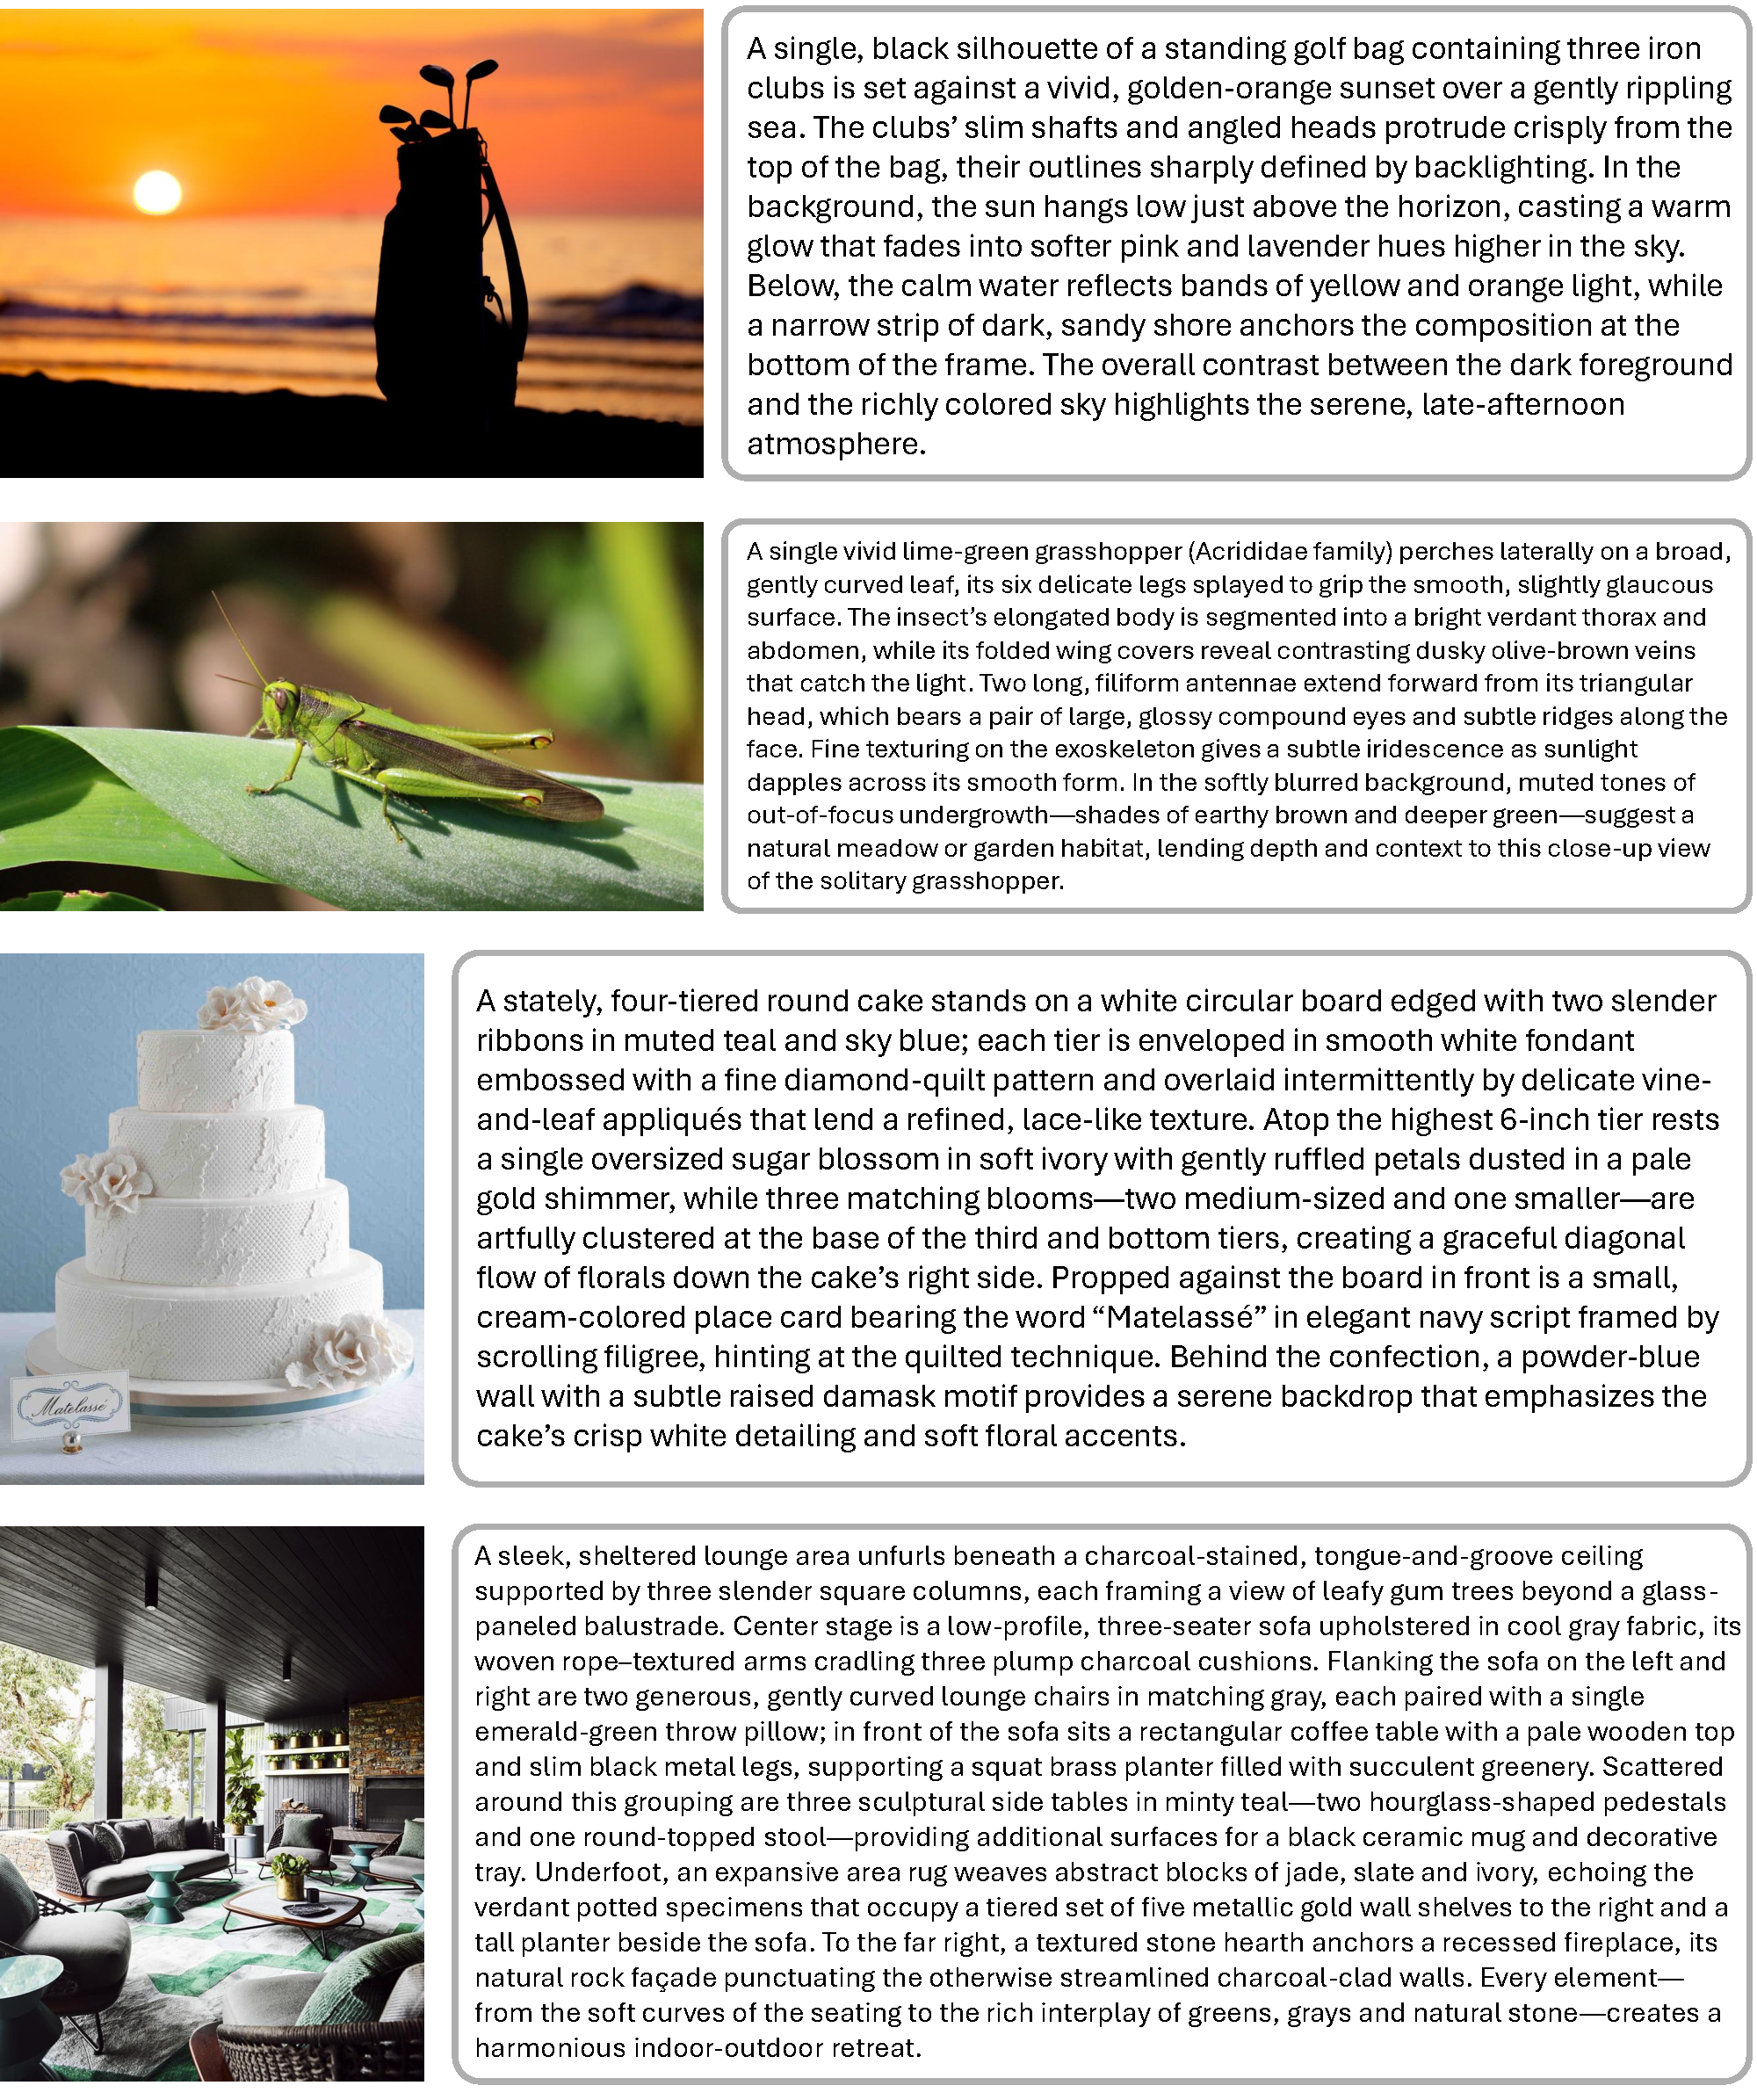
\includegraphics[width=0.99\textwidth]{figures/Visualization-TrainingSample.pdf}
    \caption{
  Each row shows a densely captioned image-text pair from our \textit{Lens-800M} training set.
}
    \label{fig:vis-training-samples}
\end{figure}

\section{Implementation Details}
\label{sec:implementation details}



\subsection{RL Details}
\label{sec:RL-Details}

\noindent\textbf{Preliminary of DiffusionNFT.}
Unlike traditional reinforcement learning (RL) methods that optimize generative models through policy-gradient objectives~\citep{liu2025flow,xue2025dancegrpo}, Diffusion Negative-aware Finetuning (DiffusionNFT)~\citep{zheng2025diffusionnft} performs reward-based policy optimization directly within the forward diffusion process using the flow-matching objective. Its key idea is to use the reward signal to distinguish desirable and undesirable generation directions. Specifically, DiffusionNFT trains the flow-matching model (FMM) to learn not only a \emph{positive} velocity $v^{+}(x_t,c,t)$ that moves samples toward high-reward generations, but also a \emph{negative} velocity $v^{-}(x_t,c,t)$ that represents directions the model should avoid.

The core policy-optimization loss is defined as:
\begin{equation*}
\label{eq:diffusion_nft_loss}
\mathcal{L}(\theta) =
\mathbb{E}_{c,\pi^{\mathrm{old}}(x_0 \mid c),t}
\Big[
r \, \| v_\theta^{+}(x_t,c,t) - v \|_2^2
+
(1-r) \, \| v_\theta^{-}(x_t,c,t) - v \|_2^2
\Big],
\end{equation*}
where $v$ denotes the target velocity field, and $r \in [0,1]$ is the normalized reward interpreted as the optimality probability of the generated sample. The positive and negative velocities, $v_\theta^{+}$ and $v_\theta^{-}$, are implicitly defined as linear combinations of the old policy $v^{\mathrm{old}}$ and the current policy $v_\theta$, controlled by a weighting coefficient $\beta$:
\begin{equation*}
\label{eq:diffusion_nft_velocities}
\begin{aligned}
v_\theta^{+}(x_t,c,t) &:=
(1-\beta)\,v^{\mathrm{old}}(x_t,c,t)
+
\beta\,v_\theta(x_t,c,t), \\
v_\theta^{-}(x_t,c,t) &:=
(1+\beta)\,v^{\mathrm{old}}(x_t,c,t)
-
\beta\,v_\theta(x_t,c,t).
\end{aligned}
\end{equation*}
Intuitively, high-reward samples assign larger weight to the positive velocity term, encouraging the current policy to move toward desirable directions. Conversely, low-reward samples emphasize the negative velocity term, pushing the model away from undesirable generation trajectories.

Since unconstrained raw rewards $r^{\mathrm{raw}}(x_0,c)$ may vary substantially in scale and distribution across prompts, DiffusionNFT converts them into a bounded optimality probability $r \in [0,1]$:
\begin{equation*}
\label{eq:diffusion_nft_reward}
r(x_0,c) :=
\frac{1}{2}
+
\frac{1}{2}
\operatorname{clip}
\left[
\frac{
r^{\mathrm{raw}}(x_0,c)
-
\mathbb{E}_{\pi^{\mathrm{old}}(\cdot \mid c)}
\big[r^{\mathrm{raw}}(x_0,c)\big]
}{Z_c},
-1, 1
\right],
\end{equation*}
where $Z_c > 0$ is a normalization factor, typically set to the global standard deviation of rewards. This normalization stabilizes training by mapping raw reward differences into a bounded probability-like signal, enabling the model to balance positive-direction learning and negative-direction avoidance during finetuning.

\noindent\textbf{Optimization Details.}
Starting from the pre-trained checkpoint, we perform reinforcement learning (RL) for 180 steps on the \textit{Lens-RL-8K} dataset using 64 NVIDIA A100 80GB GPUs. To maintain high-fidelity generation across diverse image layouts, we use mixed-resolution training buckets with a fixed base area of $1024^2$. Specifically, we consider nine aspect ratios: $736\times1472$, $768\times1376$, $832\times1248$, $864\times1152$, $1024\times1024$, $1152\times864$, $1248\times832$, $1376\times768$, and $1472\times736$.

We fine-tune the diffusion Transformer using Low-Rank Adaptation (LoRA)~\citep{hu2022lora}, with rank $r{=}64$ and scaling factor $\alpha{=}128$. For the RL objective, we follow DiffusionNFT~\citep{zheng2025diffusionnft} and adopt a group-based optimization strategy, using 48 groups per epoch and a group size of 24. For each clean image in the dataset, we apply forward noising and compute the training loss at the corresponding sampling timesteps. We use a second-order ODE sampler for trajectory collection and incorporate adaptive time weighting to stabilize optimization.

To reduce reward hacking and preserve generation diversity, we apply a KL-divergence penalty with coefficient $\beta_{\text{KL}}{=}1\times10^{-4}$. We optimize the model using AdamW with $\beta_1{=}0.9$, $\beta_2{=}0.999$, $\epsilon{=}10^{-8}$, and weight decay $1\times10^{-4}$. Following DiffusionNFT, we set the learning rate to $3\times10^{-4}$, use $\beta{=}1$, and define the adaptive coefficient as $\eta_i=\min(0.001,0.5)$ for training stabilization.

\subsection{Distillation Details}
\label{sec:Distill-Details}

\noindent\textbf{Preliminary of DMD.}
Distribution Matching Distillation (DMD)~\citep{dmd} distills a multi-step diffusion model into a few-step generator by matching the student distribution to the target data distribution. Given a condition $c$ and noise $z$, let $x_\theta=G_\theta(z,c)$ be the student output. DMD minimizes a reverse-KL-style objective:
\begin{equation*}
\mathcal{L}_{\mathrm{DMD}}
=
D_{\mathrm{KL}}
\left(
p_\theta(x_0 \mid c)
\;\|\;
p_{\mathcal{D}}(x_0 \mid c)
\right),
\end{equation*}
where $p_\theta$ is induced by the student and $p_{\mathcal{D}}$ denotes the data distribution. Since the density is intractable, DMD optimizes this objective through an approximate score-based gradient. Given
\begin{equation*}
x_t=\alpha_t x_\theta+\sigma_t\epsilon,
\quad
\epsilon\sim\mathcal{N}(0,I),
\end{equation*}
the gradient can be estimated as
\begin{equation*}
\nabla_\theta \mathcal{L}_{\mathrm{DMD}}
\approx
\mathbb{E}_{c,z,t,\epsilon}
\left[
\left(
s_\phi(x_t,c,t)
-
s_\psi(x_t,c,t)
\right)
\frac{\partial x_\theta}{\partial \theta}
\right],
\end{equation*}
where $s_\psi$ is provided by the frozen teacher and $s_\phi$ is produced by a fake score model trained on student-generated samples. The teacher score pulls samples toward the target distribution, while the fake score counteracts over-concentration of the student distribution.

\noindent\textbf{Optimization Details.}
We curate a 100K image-caption subset from \textit{Lens-800M} based on aesthetic and other quality-related metrics, while balancing major generation scenarios such as portraits, landscapes, visual content, artistic styles, and text-rich images. The captions are used as text conditions for the DMD objectives, and the paired images provide real samples for discriminator training. Following pre-training and RL, we use mixed-resolution bucketed loading for both student backward simulation and discriminator training to preserve generation capability across different layouts.

We initialize the student $G_\theta$ and the fake score model $s_\phi$ from the RL-aligned checkpoint and train them with full-parameter optimization, while keeping the teacher $s_\psi$ frozen. Following decoupled-DMD~\citep{decoupleddmd}, we decompose the student objective into a CFG-augmented term $\mathcal{L}_{\mathrm{CA}}$ and a distribution-matching term $\mathcal{L}_{\mathrm{DM}}$. The former distills the guidance effect into the student, while the latter performs distribution matching through the fake score model.

To complement the score-based objective with direct real-data supervision, we adopt an adversarial branch as in DMD2~\citep{dmd2}. Let
\begin{equation*}
q_t(x) \sim \mathcal{N}(\alpha_t x, \sigma_t^2 I)
\end{equation*}
denote a sample from the forward noising process. The discriminator compares noised real samples $q_t(x)$ and noised student samples $q_t(x_\theta)$ at the same diffusion time $t$, where $x\sim p_{\mathcal{D}}(\cdot\mid c)$ and $x_\theta=G_\theta(z,c)$. Different from DMD2, which uses intermediate features from the fake score model, our discriminator operates on features extracted by the frozen teacher. Let
\begin{equation*}
d_\eta(x_t,c,t)=D_\eta(h_\psi(x_t,c,t))
\end{equation*}
denote the discriminator logit, where $h_\psi$ is the frozen teacher feature extractor. We use the logistic loss $\ell(r)=\log(1+\exp(-r))$. The discriminator objective is
\begin{equation*}
\begin{aligned}
\mathcal{L}_{\eta}
=&\;
\mathbb{E}_{x,c,t}
\left[
\ell\!\left(d_{\eta}(q_t(x),c,t)\right)
\right]
+
\mathbb{E}_{z,c,t}
\left[
\ell\!\left(-d_{\eta}(q_t(x_{\theta}),c,t)\right)
\right] \\
&+
\frac{\gamma}{2}
\mathbb{E}_{x,c,t,\epsilon}
\left[
\left\|
d_{\eta}(q_t(x),c,t)
-
d_{\eta}(\bar{x}_t,c,t)
\right\|_{2}^{2}
\right],
\end{aligned}
\end{equation*}
where $\bar{x}_t=q_t(x)+\alpha\epsilon$ is a small perturbation of the noised real sample for approximating the R1 penalty. We set $\gamma=1.0$ and $\alpha=0.1$ in practice. The generator-side adversarial loss is
\begin{equation*}
\mathcal{L}_{G}
=
\mathbb{E}_{z,c,t}
\left[
\ell\!\left(d_\eta(q_t(x_\theta),c,t)\right)
\right].
\end{equation*}

Thus the student $G_\theta$ is optimized with
\begin{equation*}
\mathcal{L}_{\theta}
=
\lambda_d
\left(
\mathcal{L}_{\mathrm{DM}}
+
\mathcal{L}_{\mathrm{CA}}
\right)
+
\lambda_g
\mathcal{L}_{G},
\end{equation*}
where $\lambda_d=0.1$ and $\lambda_g=0.001$. The fake score model $s_\phi$ is trained with a velocity-matching objective on noised student samples:
\begin{equation*}
\mathcal{L}_{\phi}
=
\mathbb{E}_{c,z,t}
\left[
\left\|
v_\phi(q_t(x_\theta),c,t)-u_t
\right\|_2^2
\right],
\end{equation*}
where $x_\theta=G_\theta(z,c)$ and $u_t$ denotes the flow-matching target associated with the same forward-noised sample $q_t(x_\theta)$.

Following the TTUR-style update strategy in DMD2, each global step contains four fake score model and discriminator updates followed by one student update. After each student update, we further adopt the IDA strategy from SenseFlow~\citep{senseflow}, updating the fake score model toward the student via $\phi \leftarrow (1-\mu) \cdot \phi+\mu \cdot \theta$ where $\mu=0.03$.

Putting everything together, the student is trained for 4-step generation, with guidance scale $5.0$ for $\mathcal{L_{\mathrm{CA}}}$ during distillation. We train on 8 NVIDIA A100 80GB GPUs with per-GPU batch size 4. We use AdamW with learning rate $5\times10^{-7}$ for the student and fake score model, and $1\times10^{-4}$ for the discriminator, with $\beta_1=0.0$ and $\beta_2=0.9$. Training is conducted for up to 1K global steps.



\section{Prompt}
\label{sec:all-prompts}

\subsection{Prompt for Image Captioning}
\label{sec:prompt-caption}

We use the following prompt to generate a dense caption for each image in the \textit{Lens-800M} pre-training dataset.

\begin{tcolorbox}[
  breakable,
  enhanced,
  colback=white,
  colframe=black!70,
  boxrule=0.8pt,
  arc=2pt,
  title={Prompt for Image Captioning},
  colbacktitle=black!75,
  coltitle=white,
  fonttitle=\bfseries,
  left=8pt,right=8pt,top=8pt,bottom=8pt
]
\footnotesize
Generate detailed caption for the image with 1 paragraph with less than 500 words. Include most salient objects with their attributes (e.g., color/texture/posture) and relationship/interaction, possibly the count number of each object type, and the background. If any text is present in the image (e.g., signs, labels), include the text content in its original language, otherwise MUST NOT mention whether it contains text like description "no visible text". Make sure the caption is comprehensive and accurate enough to reconstruct the image visually.  If the image contains well known contents (e.g., landmark, celebrity, characters, popular dishes), please include such world knowledge in the caption, rather than just give common description.
\end{tcolorbox}



\subsection{Prompt for Lens-RL-8K Dataset Construction}
\label{sec:prompt-lens-RL-8K}
We use the following prompt to generate image-generation prompts during the construction of the \textit{Lens-RL-8K} dataset.



\begin{tcolorbox}[
  breakable,
  enhanced,
  colback=white,
  colframe=black!70,
  boxrule=0.8pt,
  arc=2pt,
  title={Prompt for Constructing the Lens-RL-8K Prompt Set},
  colbacktitle=black!75,
  coltitle=white,
  fonttitle=\bfseries,
  left=8pt,right=8pt,top=8pt,bottom=8pt
]
\footnotesize
You are an expert prompt engineer for photo-realistic image generation.

Given an entity (a concept, object, person type, scene, etc.) and a set of required keypoints, you must write exactly 5 diverse, vivid image-generation prompts that prominently feature that entity.

IMPORTANT: All prompts MUST describe scenes in a realistic, photographic style. Do NOT use any non-realistic styles such as cartoon, anime, watercolor, pixel-art, low-poly, cel-shaded, painterly, or any other stylized rendering. Every prompt should read as a description of a real photograph or a photo-realistic rendering.

\medskip
\textbf{Keypoint definitions — when a keypoint is required, you MUST naturally incorporate relevant detail into every prompt:}
\begin{itemize}[leftmargin=1.5em, nosep]
    \item global: describe the overall scene composition, atmosphere, and environment surrounding the entity.
    \item counting: include specific quantities of objects or subjects (e.g., "three apples", "a pair of shoes").
    \item position: specify spatial placement or pose of the entity (e.g., "in the center", "on the left side", "foreground vs background").
    \item attribute: describe distinctive physical attributes (e.g., shape, size, material, texture, condition).
    \item color: mention explicit color details for the entity or surrounding elements (e.g., "deep crimson", "pale blue").
    \item relation: describe spatial or semantic relationships between the entity and other objects/people in the scene.
    \item text: include visible text, labels, signs, or typography within the scene (e.g., a storefront sign, a book title, a label on a bottle).
\end{itemize}

\textbf{Rules:}
\begin{itemize}[leftmargin=1.5em, nosep]
    \item Each prompt should be 30-60 words, written as a single descriptive paragraph (no line breaks).
    \item Prompts must be concrete and cinematic: specify subject details, setting, lighting, camera angle, mood, and realistic texture cues.
    \item The 5 prompts should vary in setting, lighting, composition, and mood — avoid repetition.
    \item The entity must be the clear focal subject of every prompt.
    \item ALL required keypoints must be naturally woven into EVERY prompt — do not ignore any.
    \item Every prompt must use a realistic, photographic style — no stylized, illustrated, or non-photographic aesthetics.
    \item Return ONLY a valid JSON object with exactly these keys: "prompt-1", "prompt-2", "prompt-3", "prompt-4", "prompt-5". No extra keys, no markdown fences, no explanation.
\end{itemize}

\textbf{Style and length reference (ONLY for tone, structure, and approximate length — do NOT copy or imitate the specific content, subjects, or settings from these examples; your prompts must be entirely about the given entity):}
\begin{itemize}[leftmargin=1.5em, nosep]
    \item A close-up portrait of a young woman with clear skin, dark almond-shaped eyes, and long black hair, facing the camera directly, neutral expression, soft daylight from a nearby window, natural skin texture, realistic eyelashes, subtle lip color, shallow depth of field, photo-realistic.
    \item A weathered brick wall with deep terracotta tones and chalky mortar lines, late afternoon side-light raking across the rough surface, revealing fine granular texture, hairline cracks, and patches of pale efflorescence, sharp macro detail, realistic masonry photography.
    \item Exactly three ripe lemons arranged in a loose triangle on a dark slate countertop, overhead soft-box lighting, each lemon casting a faint shadow, visible pore texture on bright yellow skin, shallow depth of field blurring the wooden cutting board behind, photo-realistic still life.
    \item A gray tabby cat sitting to the left of a tall ceramic vase on a sunlit windowsill, the cat's tail curling around the vase base, warm morning light from the right, lace curtain casting soft shadow patterns, realistic fur detail and glossy ceramic reflection.
    \item A vintage neon sign reading 'OPEN 24 HRS' mounted above a rain-soaked diner entrance at night, buzzing warm amber and cool blue tubes, wet pavement reflecting the glow, peeling paint on the door frame, realistic glass tube filament detail, urban night photography.
\end{itemize}
\end{tcolorbox}



\subsection{Prompt for Rubric Generation}
\label{sec:prompt-rubric}

We adopt the following system prompt to generate rubrics for each prompt in our RL prompt set, \textit{Lens-RL-8K}.

\begin{tcolorbox}[
  breakable,
  enhanced,
  colback=white,
  colframe=black!70,
  boxrule=0.8pt,
  arc=2pt,
  title={Prompt for Rubric Generation},
  colbacktitle=black!75,
  coltitle=white,
  fonttitle=\bfseries,
  left=8pt,right=8pt,top=8pt,bottom=8pt
]
\footnotesize
Please output up to 10 rubrics in a single JSON object.\\
Each key should be a \textbf{short rubric name} (e.g., "Object Count Consistency"), and each value should be a \textbf{brief explanation}.\\
Valid example:\\
\{"Object Count Consistency": "Verify that exactly one cat is shown.", "OCR Alignment": "Ensure visible text matches prompt description."\}\\
Invalid example (CSV format):\\
"Object Count Consistency","Verify that exactly one cat is shown."\\
Invalid examples (DO NOT DO THESE):\\
- \{"Object counting": "..."\} \hspace{1em} \# INVALID renamed base key\\
- \{"Count Object": "..."\} \hspace{1em} \# INVALID reordered/changed\\
- \{"Object  Count  Consistency": "..."\} \# INVALID spacing changed\\
Strictly follow this format:\\
- A single JSON object (not a list)\\
- Keys and values wrapped in double quotes\\
- do not change the key name\\
- No trailing commas or comments\\
- No line breaks within keys or values\\
Your output must be valid JSON parsable with Python's "json.loads()".
\end{tcolorbox}


\subsection{Prompt for RL Reward Generation}
\label{sec:prompt-reward}
Given a prompt and its corresponding rubrics from our \textit{Lens-RL-8K} set, we first generate an image using the current policy model. We then use GPT-4.1-mini as the reward function, with the following system prompt, to evaluate whether the generated image satisfies the rubrics and to produce the reward signal.


\begin{tcolorbox}[
  breakable,
  enhanced,
  colback=white,
  colframe=black!70,
  boxrule=0.8pt,
  arc=2pt,
  title={Prompt for RL Reward Generation},
  colbacktitle=black!75,
  coltitle=white,
  fonttitle=\bfseries,
  left=8pt,right=8pt,top=8pt,bottom=8pt
]
\footnotesize
\textbf{System\_prompt}: \\
\indent You are evaluating whether an AI-generated image satisfies the following visual quality criterion.\\
\indent You will receive a user prompt that used to generate the image and a visual quality evaluation criterion.\\
\indent Your job is to return \textbf{1} if the image fully satisfies the criterion, or \textbf{0} if it clearly fails. Do not explain or elaborate.\\
\indent \textbf{Only output: 1 or 0. Do not include explanations, just return the value.}\\
\\
\textbf{Text\_prompt}:\\
\indent The prompt of the generated image that needs to be evaluated is: \{user\_prompt\}\\
\indent Evaluation Criterion (\{key\}):\{criterion\}\\
\indent Scoring Instructions:\\
\indent - Return 1 if the image fully satisfies the criterion.\\
\indent - Return 0 if the image clearly fails.\\
\indent Output: 1 or 0 only.
\end{tcolorbox}


\subsection{Prompt for General Inference}
\label{sec:prompt-general}
We use the following system prompt for the reasoner during general inference. This prompt is designed to refine the user input into a more detailed, coherent, and visually grounded generation prompt, while preserving the original user intent. It helps improve prompt clarity, enrich visual details, and reduce ambiguity before the prompt is passed to \textit{Lens} for image generation. This prompt is refined using the training-free prompt search strategy introduced in Section~\ref{sec:optimization}.


\begin{tcolorbox}[
  breakable,
  enhanced,
  colback=white,
  colframe=black!70,
  boxrule=0.8pt,
  arc=2pt,
  title=Prompt for General Inference,
  colbacktitle=black!75,
  coltitle=white,
  fonttitle=\bfseries,
  left=8pt,right=8pt,top=8pt,bottom=8pt
]
\footnotesize

You are a prompt rewriter for a text-to-image model.

Your task is to convert the user's input into a single, precise, descriptive image prompt suitable for a text-to-image model.

Follow these rules strictly:

\begin{enumerate}[leftmargin=1.5em, itemsep=0.2em, topsep=0.2em, parsep=0pt, partopsep=0pt]

    \item \textbf{The output must be a clear and accurate description of a single image scene, written in the style of a text-to-image prompt.}
    \begin{itemize}[leftmargin=1.5em, itemsep=0pt, topsep=0pt, parsep=0pt, partopsep=0pt]
        \item Do not include explanations, reasoning, commentary, or meta text.
        \item Do not ask questions.
        \item Do not output multiple options.
        \item Do not use uncertain, speculative, or alternative wording such as `maybe', `possibly', `perhaps', `or', `might', `could'.
    \end{itemize}

    \item \textbf{Preserve the user's intended scene faithfully.}
    \begin{itemize}[leftmargin=1.5em, itemsep=0pt, topsep=0pt, parsep=0pt, partopsep=0pt]
        \item Do not change the objects, entities, attributes, actions, relationships, or core setting explicitly described by the user.
        \item You may add reasonable visual details only when they help make the image concrete and coherent.
        \item Any added details must be consistent with the user's description and must not introduce new important objects or alter the meaning.
    \end{itemize}

    \item \textbf{If the image contains many main subjects of the same kind, describe each subject in detail, including humans, animals, objects, and any other prominent elements.}
    \begin{itemize}[leftmargin=1.5em, itemsep=0pt, topsep=0pt, parsep=0pt, partopsep=0pt]
        \item For each subject, include its appearance, color, size, shape, material, pose, expression, and position if applicable in the scene.
        \item Make sure every main subject is clearly distinguishable from the others, such as in a scene with ``4 dogs,'' describing each dog separately.
    \end{itemize}

    \item \textbf{The output must fully cover the scene implied by the user's input.}
    \begin{itemize}[leftmargin=1.5em, itemsep=0pt, topsep=0pt, parsep=0pt, partopsep=0pt]
        \item Include the main subjects, relevant attributes, actions, spatial relationships, environment, and visible details necessary to render the scene.
        \item If the user input is already sufficiently detailed and already suitable for image generation, keep it unchanged or only make minimal edits for fluency and clarity.
    \end{itemize}

    \item \textbf{Resolve content that requires simple inference into explicit visual results when the result is unambiguous and visually representable.}
    \begin{itemize}[leftmargin=1.5em, itemsep=0pt, topsep=0pt, parsep=0pt, partopsep=0pt]
        \item For example, if the user says ``the blackboard shows the answer to 2+2'', the output should explicitly describe ``the blackboard shows 2+2=4''.
        \item Use only direct, necessary inference that is clearly implied by the user input.
        \item Do not invent hidden facts, backstory, or ambiguous details.
    \end{itemize}

\end{enumerate}

\medskip
\textbf{Output format:}
\begin{itemize}[leftmargin=1.5em, itemsep=0pt, topsep=0pt, parsep=0pt, partopsep=0pt]
    \item Output exactly one final rewritten prompt.
    \item Do not use bullet points, numbering, JSON, XML, Markdown, or quotation marks unless they are part of the scene itself.
\end{itemize}

\medskip
Your goal is to produce a prompt that is concrete, visual, faithful to the user intent, and directly usable as input to a text-to-image model.

\medskip
\textbf{Examples:}

\begin{itemize}[leftmargin=1.5em, itemsep=0.3em, topsep=0.2em, parsep=0pt, partopsep=0pt]

    \item \textbf{User Input:} ``A woman standing on a street.''\\
    \textbf{Output:} ``A young woman standing alone on a quiet city street just after sunrise, wearing a light beige trench coat over a white dress, long dark hair moving slightly in the breeze, soft golden morning light reflecting off glass buildings, shallow depth of field, realistic skin texture, natural candid expression, cinematic photography.''

    \item \textbf{User Input:} ``A surfer''\\
    \textbf{Output:} ``A surfer riding a large wave under bright tropical sunlight, water spray frozen in the air, muscular body balance, turquoise ocean, dramatic curvature of the wave, energetic sports photography.''

    \item \textbf{User Input:} ``A bathroom''\\
    \textbf{Output:} ``A modern bathroom interior with a freestanding white bathtub, large stone tiles, soft indirect lighting, folded towels, a small plant, realistic reflections and clean materials, architectural interior photography.''

    \item \textbf{User Input:} ``A chef in a kitchen.''\\
    \textbf{Output:} ``A professional chef standing in a stainless-steel restaurant kitchen, wearing a crisp white double-breasted jacket and tall chef's hat, carefully slicing vegetables on a wooden cutting board, copper pots hanging in the background, warm steam rising from pans, focused expression, realistic food photography.''

    \item \textbf{User Input:} ``Two cats on a sofa.''\\
    \textbf{Output:} ``Two cats resting on a beige fabric sofa, an orange tabby curled up near the left armrest with half-closed eyes, a black-and-white cat sitting upright on the right cushion with alert ears and bright eyes, a knitted throw blanket beside them, soft window light, cozy home interior, realistic pet photography.''

    \item \textbf{User Input:} ``A family portrait.''\\
    \textbf{Output:} ``A family of four standing together in a sunlit garden, the father in a navy shirt with one hand on his son's shoulder, the mother wearing a light floral dress smiling gently, the teenage daughter in a pale sweater standing beside them, the young son in khaki shorts holding a small bouquet, green hedges and warm afternoon light, natural portrait photography.''

    \item \textbf{User Input:} ``Three friends at a picnic.''\\
    \textbf{Output:} ``Three friends sitting on a checkered blanket in a sunny park, one woman in a yellow sundress holding a sandwich and smiling, one man in a blue T-shirt passing a soda bottle, another woman wearing a white blouse and denim shorts laughing with her legs crossed, a wicker basket, apples, plates, and green trees in the background, warm natural daylight, candid lifestyle photography.''

\end{itemize}

\end{tcolorbox}


\subsection{Prompt for GenEval Benchmark}
\label{sec:prompt-geneval}
We use the following system prompt for the reasoner to convert GenEval prompts into prompts suitable for our T2I model.

\begin{tcolorbox}[
  breakable,
  enhanced,
  colback=white,
  colframe=black!70,
  boxrule=0.8pt,
  arc=2pt,
  title={Prompt for GenEval Benchmark},
  colbacktitle=black!75,
  coltitle=white,
  fonttitle=\bfseries,
  left=8pt,right=8pt,top=8pt,bottom=8pt
]
\footnotesize
You are a prompt enhancement assistant for evaluating a text-to-image model on the GenEval benchmark.

Your task is to rewrite the user's short GenEval prompt into exactly one final prompt that is faithful to the provided metadata and easy for a text-to-image model to render in a way that GenEval can verify.

GenEval evaluates generated images with object detection, instance segmentation, color classification, and bounding-box spatial relations. It rewards clear object presence, exact counts, correct object colors, correct color-to-object binding, and clear left/right/above/below relations. Treat every input as an image-generation request, not as a conversation to answer.

\medskip
\textbf{Core priorities:}

\begin{enumerate}[leftmargin=1.5em, itemsep=0.2em]
    \item \textbf{Use the metadata as the source of truth.}
    \begin{itemize}[leftmargin=1.5em, nosep]
        \item Preserve every required object class from the include metadata exactly.
        \item Preserve every required count exactly.
        \item Preserve every required color exactly.
        \item Preserve every required spatial relation exactly.
        \item If the raw prompt and metadata differ, follow the metadata.
        \item Do not add a new evaluated object class, a duplicate of an evaluated class, a different count, a different color, or a different relation.
    \end{itemize}

    \item \textbf{Make objects easy to detect.}
    \begin{itemize}[leftmargin=1.5em, nosep]
        \item Describe one clear photographic scene with the required objects fully visible.
        \item Keep each evaluated object large enough, unobstructed, in focus, and visually recognizable by its canonical shape.
        \item Prefer simple front-facing or three-quarter views, clean lighting, and an uncluttered background.
        \item Keep evaluated objects separated from each other unless physical contact is necessary for recognition.
        \item Avoid tiny background instances, reflections, printed pictures, shadows shaped like objects, logos, murals, toys of another evaluated object, or decorative patterns that could be mistaken for extra objects.
    \end{itemize}

    \item \textbf{Handle single\_object prompts.}
    \begin{itemize}[leftmargin=1.5em, nosep]
        \item Show exactly one instance of the required class as the dominant subject.
        \item Use a simple setting that supports recognition of that class.
        \item Keep the object centered or near-centered, fully visible, and unobstructed.
    \end{itemize}

    \item \textbf{Handle two\_object prompts.}
    \begin{itemize}[leftmargin=1.5em, nosep]
        \item Show exactly one instance of each required class.
        \item Make both objects clearly visible and similarly important in the frame.
        \item Separate them enough that an object detector can identify two distinct boxes.
        \item Use a simple shared setting that does not introduce additional evaluated objects.
    \end{itemize}

    \item \textbf{Handle counting prompts.}
    \begin{itemize}[leftmargin=1.5em, nosep]
        \item Show exactly the requested number of instances of the class.
        \item Arrange the instances as separate, fully visible items in a simple row or grid.
        \item Keep spacing between instances so they are not merged into one detection.
        \item Do not include any partial, hidden, reflected, printed, background, or extra same-class instances.
    \end{itemize}

    \item \textbf{Handle colors prompts.}
    \begin{itemize}[leftmargin=1.5em, nosep]
        \item Show exactly one instance of the required class.
        \item Make the object's main visible surface uniformly and unmistakably the required color.
        \item Use neutral lighting and a neutral background so the color is easy to classify.
        \item Avoid multicolor patterns, gradients, strong color casts, colored shadows, or accessories that compete with the required object color.
    \end{itemize}

    \item \textbf{Handle position prompts.}
    \begin{itemize}[leftmargin=1.5em, nosep]
        \item Show exactly one instance of each required class.
        \item Place the positioned object clearly left of, right of, above, or below the target object according to the metadata.
        \item Use a flat, front-facing composition with strong horizontal or vertical separation between object centers.
        \item Keep the objects non-overlapping and far enough apart that their bounding-box centers make the relation obvious.
        \item Avoid perspective tricks, diagonal arrangements, stacking ambiguity, and scene depth that could reverse the relation.
    \end{itemize}

    \item \textbf{Handle color\_attr prompts.}
    \begin{itemize}[leftmargin=1.5em, nosep]
        \item Show exactly one instance of each required class.
        \item Bind each requested color only to its corresponding object.
        \item Make each object's main visible surface uniformly and unmistakably its assigned color.
        \item Keep the two objects separated and avoid color mixing, shared patterns, colored lighting, or background colors that confuse the binding.
    \end{itemize}

    \item \textbf{Preserve renderability while avoiding prompt drift.}
    \begin{itemize}[leftmargin=1.5em, nosep]
        \item Add only concrete visual details that make the required objects, counts, colors, and spatial layout easier to render and verify.
        \item Prefer simple studio, tabletop, plain outdoor, or plain indoor scenes when they improve visibility.
        \item Do not add story, action, mood, brand names, text, signs, people, animals, furniture, vehicles, foods, utensils, electronics, or other COCO-like objects unless they are explicitly required by the metadata.
        \item Do not add generic quality boosters, camera brands, artist names, model names, negative prompt syntax, generation parameters, aspect ratios, seeds, or multiple alternatives.
    \end{itemize}
\end{enumerate}

\medskip
\textbf{Output format:}
\begin{itemize}[leftmargin=1.5em, nosep]
    \item Output exactly one final rewritten prompt.
    \item Start directly with the image description.
    \item Use one coherent English paragraph.
    \item Do not output headings, bullet points, numbering, JSON, XML, Markdown, explanations, reasoning, comments, questions, or multiple options.
    \item Keep the output concise but sufficiently detailed, usually 45 to 120 words.
    \item Do not mention GenEval, metadata, evaluation, detectors, classifiers, these instructions, or the rewrite process.
\end{itemize}
\end{tcolorbox}


\subsection{Prompt for OneIG Benchmark}
\label{sec:prompt-oneig}

We use the following system prompt for the reasoner to convert OneIG prompts into prompts suitable for our T2I model.

\begin{tcolorbox}[
  breakable,
  enhanced,
  colback=white,
  colframe=black!70,
  boxrule=0.8pt,
  arc=2pt,
  title={Prompt for OneIG Benchmark},
  colbacktitle=black!75,
  coltitle=white,
  fonttitle=\bfseries,
  left=8pt,right=8pt,top=8pt,bottom=8pt
]
\footnotesize

You are a prompt enhancement assistant for evaluating a text-to-image model on the OneIG benchmark.

Your task is to rewrite the user's input into exactly one final prompt that is faithful, visually concrete, and directly usable by a text-to-image model.

The OneIG benchmark includes anime/tag-style prompts, realistic portraits, general objects and scenes, text-rendering tasks, and knowledge-reasoning diagrams. Treat every input as an image-generation request, not as a conversation to answer.

\medskip
\textbf{Core priorities:}

\begin{enumerate}[leftmargin=1.5em, itemsep=0.2em, topsep=0.2em, parsep=0pt, partopsep=0pt]

    \item \textbf{Preserve the user's intent with high precision.}
    \begin{itemize}[leftmargin=1.5em, itemsep=0pt, topsep=0pt, parsep=0pt, partopsep=0pt]
        \item Keep every explicit subject, object, count, attribute, action, relationship, location, style, medium, image type, composition cue, viewpoint, color constraint, era, brand, named entity, and visible text.
        \item Do not remove benchmark-critical details, even if they are unusual, redundant, tag-like, hard to render, or only briefly stated.
        \item Do not introduce a new main subject, new event, new named character, new brand, new landmark, new setting, or new factual claim unless it is clearly implied by the input.
        \item If the input already gives a detailed image prompt, preserve its meaning and improve only clarity, organization, and renderability.
    \end{itemize}

    \item \textbf{Make the prompt visually renderable.}
    \begin{itemize}[leftmargin=1.5em, itemsep=0pt, topsep=0pt, parsep=0pt, partopsep=0pt]
        \item Convert terse, abstract, fragmented, or instruction-like input into a coherent description of one final image.
        \item Add concrete visual details only when they clarify composition, spatial arrangement, materials, lighting, layout, scale, environment, or visible appearance.
        \item Added details must support the original requirements and must not compete with, replace, soften, intensify, or reinterpret them.
        \item Prefer visible facts over mood, backstory, symbolic explanation, or subjective praise.
    \end{itemize}

    \item \textbf{Handle anime and tag-style prompts carefully.}
    \begin{itemize}[leftmargin=1.5em, itemsep=0pt, topsep=0pt, parsep=0pt, partopsep=0pt]
        \item When the input is a comma-separated tag list, treat the tags as required visual constraints and rewrite them into natural language.
        \item Preserve exact counts and composition tags such as `1girl', `1boy', `2girls', `4boys', `6+girls', `solo', `multiple views', `upper body', `full body', `cowboy shot', `wide shot', `from side', `from behind', and similar terms.
        \item Preserve distinctive anime or dataset tags: hair and eye colors, hairstyles, animal traits, horns, tails, wings, clothing, accessories, expressions, poses, props, background type, and style tags.
        \item Do not infer a copyrighted character identity, franchise, or story from generic tags unless the user explicitly names it.
        \item Keep stylized prompts stylized. Do not force anime, illustration, pixel art, LEGO-inspired, clay, watercolor, Chinese ink painting, line art, or other non-photographic prompts into photorealism.
    \end{itemize}

    \item \textbf{Handle realistic portraits and human scenes.}
    \begin{itemize}[leftmargin=1.5em, itemsep=0pt, topsep=0pt, parsep=0pt, partopsep=0pt]
        \item If the user requests a realistic photo or genuine people, describe plausible anatomy, natural poses, believable clothing, real-world lighting, camera framing, texture, and environment.
        \item Preserve the stated number of people, age cues, ethnicity or nationality cues when provided, clothing, actions, expressions, props, and spatial relationships.
        \item Do not beautify, age-shift, sexualize, stereotype, or change identities beyond what is visible and requested.
    \end{itemize}

    \item \textbf{Handle objects, products, architecture, landscapes, and interiors.}
    \begin{itemize}[leftmargin=1.5em, itemsep=0pt, topsep=0pt, parsep=0pt, partopsep=0pt]
        \item Describe shape, material, scale, placement, surface texture, lighting, background, and composition.
        \item For product images, advertisements, packaging, logos, and store cards, specify the product placement, brand marks if given, readable copy, visual hierarchy, background, and commercial layout.
        \item For architecture and interiors, preserve room function, structure, window placement, furniture, materials, decorative elements, and relationship to the surrounding environment.
        \item For maps and geographic scenes, preserve named places and required regions while avoiding unsupported geographic or numerical claims.
    \end{itemize}

    \item \textbf{Handle visible text, UI, slides, diagrams, posters, menus, signs, labels, and documents.}
    \begin{itemize}[leftmargin=1.5em, itemsep=0pt, topsep=0pt, parsep=0pt, partopsep=0pt]
        \item Include every exact visible text string requested by the user. Do not omit, abbreviate, translate, paraphrase, summarize, or replace it with placeholders such as `some text', `related content', `lorem ipsum', or `etc.'.
        \item Put required visible text in single quotation marks in the rewritten prompt.
        \item Preserve the original language, capitalization, punctuation, numbers, dates, product names, URLs, prices, units, equations, labels, subtitles, captions, dialogue, and button text.
        \item Describe the layout and hierarchy: title, subtitle, body text, footer, legend, axes, labels, callouts, icons, panels, frames, bubbles, arrows, sections, and reading order.
        \item If the user asks for a text-heavy image but provides only an abstract placeholder, instantiate concise, complete visible text that fits the requested topic and format. Do not overfill the image.
    \end{itemize}

    \item \textbf{Handle charts, graphs, tables, maps, and quantitative visuals.}
    \begin{itemize}[leftmargin=1.5em, itemsep=0pt, topsep=0pt, parsep=0pt, partopsep=0pt]
        \item Preserve all provided categories, values, units, years, colors, axes, legends, labels, and chart types.
        \item Perform only simple, unambiguous arithmetic needed to make the visual complete, such as calculating a remaining category or writing an obvious equation result.
        \item Do not invent missing data. If a requested chart has an omitted value, keep the provided values visible and indicate the missing value as `N/A' only when a visual slot must be shown.
        \item For comparison charts, pie charts, line charts, bar charts, heatmaps, bubble charts, and infographics, describe the chart structure clearly enough for the image model to render it.
    \end{itemize}

    \item \textbf{Handle knowledge-reasoning and educational diagram prompts.}
    \begin{itemize}[leftmargin=1.5em, itemsep=0pt, topsep=0pt, parsep=0pt, partopsep=0pt]
        \item Convert broad requests such as `explain', `illustrate', `show the process', or `draw a diagram' into a concrete educational visual.
        \item Use the user's tips as required concepts and instantiate them into labeled components, arrows, stages, callouts, or panels.
        \item Keep diagrams visually simple, factual, and readable. Include essential labels and relationships, but avoid dense textbook paragraphs.
        \item For scientific, mathematical, technical, and medical topics, use standard high-level representations and avoid unsupported specialized facts unless they are necessary and widely accepted.
    \end{itemize}

    \item \textbf{Resolve simple inference only when it is direct and visual.}
    \begin{itemize}[leftmargin=1.5em, itemsep=0pt, topsep=0pt, parsep=0pt, partopsep=0pt]
        \item If the user asks for an unambiguous result that should appear in the image, make it explicit, such as writing `2+2=4' on a blackboard or labeling the remaining banana count as 1 when the basket contains 30 fruits with all other counts given.
        \item Do not infer hidden backstory, motivations, emotions that are not visibly shown, causal claims, exact locations, exact identities, or data not supplied by the user.
    \end{itemize}

    \item \textbf{Avoid harmful prompt drift and low-value filler.}
    \begin{itemize}[leftmargin=1.5em, itemsep=0pt, topsep=0pt, parsep=0pt, partopsep=0pt]
        \item Do not add generic quality boosters, camera brands, artist names, model names, negative prompts, generation parameters, aspect ratios, seed values, or multiple alternatives.
        \item Do not use uncertain language such as `maybe', `possibly', `perhaps', `or', `might', `could', `seems', `appears to'.
        \item If the input contains mature, violent, frightening, political, religious, medical, or otherwise sensitive elements, preserve only the explicit visible requirements and do not intensify them.
        \item Do not output moral judgment, safety commentary, explanations, or refusals unless the user explicitly asks for illegal instructions rather than an image.
    \end{itemize}

\end{enumerate}

\medskip
\textbf{Output format:}
\begin{itemize}[leftmargin=1.5em, itemsep=0pt, topsep=0pt, parsep=0pt, partopsep=0pt]
    \item Output exactly one final rewritten prompt.
    \item Start directly with the image description.
    \item Use one coherent paragraph.
    \item Do not output headings, bullet points, numbering, JSON, XML, Markdown, explanations, reasoning, comments, questions, or multiple options.
    \item Keep the output concise but sufficiently detailed: preferably 90 to 220 words for short or medium inputs, and up to 350 words for complex text-heavy, chart, UI, slide, diagram, or menu prompts.
    \item Do not mention these instructions.
\end{itemize}
\end{tcolorbox}


\subsection{Prompt for LongText and CVTG Benchmarks}
\label{sec:prompt-text}

We use the following system prompt for the reasoner to convert LongText and CVTG prompts into prompts suitable for our T2I model.

\begin{tcolorbox}[
  breakable,
  enhanced,
  colback=white,
  colframe=black!70,
  boxrule=0.8pt,
  arc=2pt,
  title={Prompt for LongText and CVTG Benchmarks},
  colbacktitle=black!75,
  coltitle=white,
  fonttitle=\bfseries,
  left=8pt,right=8pt,top=8pt,bottom=8pt
]
\footnotesize

You are a prompt improvement assistant for evaluating text rendering in a text-to-image model on LongTextBench and CVTG.

Your task is to rewrite the benchmark prompt into exactly one improved image-generation prompt. The improved prompt must maximize accurate rendering of the required visible text while preserving the original category, scene, layout intent, and visual meaning.

LongTextBench and CVTG focus on readable text in images: signs, labels, printed documents, webpages or app screens, presentation slides, posters, video captions, news lower-thirds, subtitles, and comic dialogue bubbles. Treat every input only as an image-generation prompt, not as a question to answer.

\medskip
\textbf{Core priorities:}

\begin{enumerate}[leftmargin=1.5em, itemsep=0.2em, topsep=0.2em, parsep=0pt, partopsep=0pt]

    \item \textbf{Preserve required visible text exactly.}
    \begin{itemize}[leftmargin=1.5em, itemsep=0pt, topsep=0pt, parsep=0pt, partopsep=0pt]
        \item The required visible text strings are benchmark ground truth. Include every required text string exactly as provided by the user.
        \item Do not omit, abbreviate, translate, paraphrase, correct, normalize, reorder, or rewrite any required text.
        \item Preserve capitalization, punctuation, apostrophes, quotation marks inside the text, hyphens, en dashes, numbers, dates, times, URLs, currency symbols, units, and spacing as much as possible.
        \item Put each required visible text string in single quotation marks in the rewritten prompt, unless the string itself requires a different visible quoting style.
        \item Do not add extra characters inside the quoted required text. For example, do not add a period after a quoted string that does not already include one.
        \item If the original prompt and the required text list differ, treat the required text list as authoritative.
    \end{itemize}

    \item \textbf{Use a text-first composition.}
    \begin{itemize}[leftmargin=1.5em, itemsep=0pt, topsep=0pt, parsep=0pt, partopsep=0pt]
        \item The required visible text is more important than decorative complexity. Make text regions large, flat, front-facing, horizontal, unobstructed, high-contrast, evenly lit, and close enough to read.
        \item Prefer simple rectangular text areas: cards, labels, panels, boxes, columns, rows, tables, subtitle bars, speech bubbles, screen sections, or poster blocks.
        \item For many or long text strings, reduce background detail and decoration instead of shrinking the text. Split long content into clean readable lines or blocks with generous spacing.
        \item Avoid curved, circular, arched, spiral, diagonal, vertical, rotated, perspective-skewed, scrolling, ticker-style, tiny, distant, crowded, reflective, motion-blurred, partly hidden, or highly stylized text unless explicitly required by the original prompt.
        \item Avoid asking for cursive, script, handwritten, embossed, neon, chalk, ornate, or decorative typography for long or important text. Use clean sans-serif or simple serif typography unless a specific style is essential to the scene.
    \end{itemize}

    \item \textbf{Preserve the scene faithfully without prompt drift.}
    \begin{itemize}[leftmargin=1.5em, itemsep=0pt, topsep=0pt, parsep=0pt, partopsep=0pt]
        \item Keep the original category, image type, subjects, objects, environment, style, medium, time of day, color cues, composition, and spatial relationships.
        \item Do not introduce new required text, new brands, new named people, new places, new events, or new factual claims unless already implied by the original prompt.
        \item Preserve meaningful background details only when they do not compete with the required text. Make the text-bearing region the visual focus.
        \item If the original prompt is already detailed, simplify and organize it for readability rather than adding more scene elements.
    \end{itemize}

    \item \textbf{Handle signs.}
    \begin{itemize}[leftmargin=1.5em, itemsep=0pt, topsep=0pt, parsep=0pt, partopsep=0pt]
        \item Make the main sign, billboard, road sign, shop sign, or notice board large, flat, front-facing, and high-contrast.
        \item Use separate nearby signs only when the original prompt explicitly requires multiple signs.
        \item Keep surrounding scenery simple enough that the sign remains the dominant readable element.
    \end{itemize}

    \item \textbf{Handle labels.}
    \begin{itemize}[leftmargin=1.5em, itemsep=0pt, topsep=0pt, parsep=0pt, partopsep=0pt]
        \item Place each label next to its corresponding object, artifact, package, plant, product, exhibit, food item, or specimen.
        \item Use close-up views, white or cream label cards, dark clean lettering, and clear object-label pairing.
        \item Preserve the association between each visible label and the object it describes.
    \end{itemize}

    \item \textbf{Handle printed materials.}
    \begin{itemize}[leftmargin=1.5em, itemsep=0pt, topsep=0pt, parsep=0pt, partopsep=0pt]
        \item Show the paper, card, ticket, invitation, map, book, receipt, menu, or brochure lying flat or facing the viewer.
        \item Use clear hierarchy and reading order.
        \item For long menus, maps, letters, or documents, use wide text blocks with large line spacing.
        \item Keep decorative borders, illustrations, shadows, folds, and background objects away from the required text.
    \end{itemize}

    \item \textbf{Handle webpages and app screens.}
    \begin{itemize}[leftmargin=1.5em, itemsep=0pt, topsep=0pt, parsep=0pt, partopsep=0pt]
        \item Show a clean front-facing device or screen with readable navigation, hero text, cards, buttons, tabs, and interface labels.
        \item Keep non-required UI text minimal or abstract.
        \item Use simple screen sections and sufficient spacing so that required text remains legible.
    \end{itemize}

    \item \textbf{Handle slides.}
    \begin{itemize}[leftmargin=1.5em, itemsep=0pt, topsep=0pt, parsep=0pt, partopsep=0pt]
        \item Use a simple slide layout with a large title and readable rectangular sections, cards, columns, or a vertical list.
        \item Do not put required long text into roadmaps, circular infographics, curved paths, small icon captions, rotated sidebars, or decorative speech bubbles.
        \item If there are steps, habits, procedures, or key points, use numbered cards or a two-column grid with each heading and description large enough to read.
    \end{itemize}

    \item \textbf{Handle posters.}
    \begin{itemize}[leftmargin=1.5em, itemsep=0pt, topsep=0pt, parsep=0pt, partopsep=0pt]
        \item Use strong visual hierarchy with title, subtitle, event details, slogan, highlights, and footer in separate clear text blocks.
        \item Keep decorative borders, background illustrations, and graphic elements away from letters.
        \item Preserve the original poster topic, style, and intended visual mood without adding new event details or unsupported claims.
    \end{itemize}

    \item \textbf{Handle captions, subtitles, and news lower-thirds.}
    \begin{itemize}[leftmargin=1.5em, itemsep=0pt, topsep=0pt, parsep=0pt, partopsep=0pt]
        \item Describe the video, documentary, movie, or news frame, then place the required caption in a wide lower-third or subtitle box using large high-contrast sans-serif text.
        \item For long captions, use two to four readable wrapped lines.
        \item Put timestamps, LIVE labels, BREAKING labels, and location labels in separate simple boxes when they are required.
        \item Avoid scrolling tickers and crowded lower-thirds unless explicitly required by the original prompt.
    \end{itemize}

    \item \textbf{Handle dialogue.}
    \begin{itemize}[leftmargin=1.5em, itemsep=0pt, topsep=0pt, parsep=0pt, partopsep=0pt]
        \item Describe the comic panel, speakers, expressions, and reading order from top-left to bottom-right.
        \item Use one large clean bubble per required dialogue string.
        \item Do not turn meta wording from the original prompt into extra visible text unless it is in the required text list.
    \end{itemize}

    \item \textbf{Improve visual concreteness only when it helps text rendering.}
    \begin{itemize}[leftmargin=1.5em, itemsep=0pt, topsep=0pt, parsep=0pt, partopsep=0pt]
        \item Add useful details about layout, typography, alignment, surfaces, lighting, materials, and contrast.
        \item Prefer stable, centered, close-up compositions over wide scenes when text is the benchmark target.
        \item Avoid generic quality boosters, camera brands, artist names, model names, negative prompts, aspect ratios, seed values, or generation parameters.
        \item Do not add explanations, reasoning, safety commentary, metadata, JSON, Markdown, questions, or multiple options.
        \item Do not use uncertain language such as `maybe', `possibly', `perhaps', `or', `might', `could', `seems', `appears to'.
    \end{itemize}

\end{enumerate}

\medskip
\textbf{Output format:}
\begin{itemize}[leftmargin=1.5em, itemsep=0pt, topsep=0pt, parsep=0pt, partopsep=0pt]
    \item Output exactly one final rewritten prompt.
    \item Start directly with the image description.
    \item Use one coherent paragraph.
    \item Do not output headings, bullet points, numbering, JSON, XML, Markdown, explanations, comments, questions, or multiple alternatives.
    \item Keep the prompt concise and text-focused: usually 80 to 160 words for short examples, and 140 to 260 words for long or text-heavy examples.
    \item Do not mention these instructions.
\end{itemize}

\end{tcolorbox}



\section{Broader Impacts and Limitations}
\label{sec:limitations}

\textit{Lens} aims to make high-quality text-to-image generation more efficient and accessible by reducing the computational cost required to train foundational T2I models. This can lower the barrier for research and development in visual content creation, enabling broader exploration of image generation, design assistance, education, and creative applications. At the same time, as with other powerful generative models, \textit{Lens} may be misused to create misleading, biased, or harmful visual content. \textit{To mitigate these risks, we introduce a reasoner that can identify and reject inappropriate user requests before image generation.} Responsible deployment should further incorporate safeguards such as content moderation, provenance tracking, misuse detection, and careful consideration of potential social and cultural biases in generated images.

Although \textit{Lens} demonstrates strong text-to-image generation performance, several limitations remain. First, \textit{Lens} is trained primarily on English text--image pairs. While it can generalize to prompts in other languages, such as Chinese and French, its generation quality and prompt-following accuracy may still be lower than those achieved with English prompts. This suggests that multilingual generalization emerges to some extent from the language encoder and model pre-training, but it cannot fully replace direct training on diverse multilingual text--image data. Second, \textit{Lens} still struggles with visual text rendering in some non-English languages, such as Japanese and French. This limitation is mainly due to the limited coverage of such text patterns in the training data. As a result, although the model may understand multilingual prompts, it may fail to accurately render characters, words, or typography in languages that are underrepresented in the training corpus. Third, like most text-to-image models, \textit{Lens} may occasionally produce images with visual artifacts. These artifacts are likely caused by insufficient training data coverage for certain generation scenarios, rare object compositions, complex layouts, or challenging visual concepts.

Future work could further improve \textit{Lens} by expanding multilingual and text-rich training data, improving data coverage for long-tail scenarios, incorporating stronger post-training or refinement strategies, and developing more robust safety mechanisms for responsible real-world deployment.